\documentclass{article}
\usepackage[utf8]{inputenc}
\usepackage{amsmath}
\usepackage{comment}
\usepackage{graphicx}
\usepackage{float}
\title{Assignment 4\\ Solutions of graph problems}
\date{}
\begin{document}
\maketitle
\begin{enumerate}

\item Let us assume that $G$ is not a cycle. \\
Consider the maximal path in the graph. Let the end points of the path be denoted as $v_1,v_k$ respectively. If either of the end nodes were connected to a node outside the considered path, we would have been able to extend the path and this would contradict that the considered path is maximal. Since $v_1,v_k$ are the end nodes, only one of their edges is exhausted. Given that the degree of the nodes are 2, each must be connected to a vertex within the path. Let us assume $v_1$ is connected to $v_i$, then degree of $v_i$ would be greater than 2, hence a contradiction. We can argue similarly if $v_k$ is connected to some node $v_j$ in the path. Thus, we can conclude that $v_1$ must be connected to $v_k$. Also note $k=n$ else the graph would be disconnected.




\item A vertex $v$ of a graph $G$ is called a \textit{cut-vertex} of $G$ if $\kappa(G-v) > \kappa(G)$.\\
Since $v$ is a cut vertex of $G$, let $(G-v)$ have components $C_1, C_2, \dots , C_k$ and $k > 1$. Consider any two vertices $x\in C_i$ and $y\in C_j$.
Then $(x,y) \notin E(G)$. Therefore $(x,y) \in E(\overline{G})$. Thus any two vertices in two different components of $G-v$ are connected by a direct edge in $\overline{G}-v$. Now consider any two vertices $(x,y)$ in the same component $C_i$ . If $(x,y) \notin E(G)$ then $(x,y) \in E(\overline{G})$. If $(x, y) \in E(G)$, then $(x,y) \notin E(\overline{G})$. But then, consider any node in a different component $z \in C_j$.
We have already shown that $(x, z) \in E(\overline{G}-v)$ and $(y,z) \in E(\overline{G}-v)$. Hence there is a path between $x$ and $y$ in $(\overline{G}-v)$. Thus, there is a path between any two vertices in $(\overline{G}-v)$. Hence $(\overline{G}-v)$ is connected.

\item For Petersen graph, we have, $v$ = 10 and $e$ = 15. Inspecting the graph, we see that: 

\begin{itemize}
\item Each edge is included in exactly two faces, and 
\item Each cycle has a length of 5 or greater. 
\end{itemize}
Combining these two facts yields $5r\le2v$. Putting $v=10$, we get, $r\le6$.
Now, substituting the values of $v$ and $e$ into Euler's formula 9$v-e+r=2$, we get $r$=7. 

Both the observations lead to a contradiction. Hence Petersen graph is non-planar.

\item  Assume that $G$ is a connected finite simple graph with $n$ vertices. Then every vertex in $G$ has degree between $1$ and $n-1$ (the degree of a given vertex cannot be zero since G is connected, and is at most $n-1$ since $G$ is simple). Since there are $n$ vertices in $G$ with degree between $1$ and $n-1$, the pigeonhole principle lets us conclude that there is some integer $k$ between $1$ and $n-1$ such that two or more vertices have degree $k$. Now, suppose $G$ is an arbitrary finite simple graph (not necessarily connected). If G has any connected component consisting of two or more vertices, the above argument shows that that component contains two vertices with the same degree, and therefore $G$ does as well. On the other hand, if $G$ has no connected components with more than one vertex, then every vertex in $G$ has degree zero, and so there are multiple vertices in $G$ with the same degree.

The same does not hold true for a multi-graph. A counter example is two vertices connected with an edge with one vertex having a loop.


\item  An equivalence relation is one, which is reflexive, symmetric and transitive. Let us check for these properties in the given relation $R$:

\begin{enumerate}
\item \textbf{Reflexive: } Since it is given that $aRb$ if $a=b$, the given relation is reflexive.
\item \textbf{Symmetric: } Since the given graph is undirected, if there is a path from $a$ to $b$, then there will be a path from $b$ to $a$ as well. Therefore, the given relation is symmetric.
\item \textbf{Transitive: } If $aRb$ and $bRc$, then definitely $aRc$, i.e. in an undirected graph, if there is a path from $a$ to $b$, and there is a path from $b$ to $c$, then there will also be a path from $a$ to $c$; hence the given relation is transitive.

\end{enumerate}

Therefore, $R$ is equivalence relation.

Further, an equivalence relation on a set $A$ divides the set into non-empty disjoint subsets called partitions of the set $A$. In the case of the given relation $R$, it will partition the vertex set $V$ into subsets where there will be a \textit{connected component} of the graph on the vertices present in each partition.

\item (Q6) \textit{If $(a, b)$ is part of a cycle then its removal does not disconnect G:}\\
If $G$ contains a cycle then removing any edge, say $(a,b)$, that is part of the cycle does not disconnect $G$ as any path that uses $(a,b)$ can now use the alternate route from $a$ to $b$ on the cycle. Therefore, removal of $(a,b)$ does not disconnect $G$.\\

\textit{If removal of $(a,b)$ does not disconnect $G$, then $(a,b)$ is a part of a cycle:}\\
Assume we remove the edge $(a,b)$ from $G$ (as given). Let us call the new graph $G_1$. It is given that removal of $(a,b)$ does not disconnect $G$. Hence $G_1$ must be connected and there is a path in it from $a$ to $b$. Now, when we add the edge $(a,b)$ to $G_1$, which is connected, $a,b$ should form a cycle in $G_1$.  


\item If every induced subgraph of a graph $G$ is connected, then $G$ must be a complete graph.

\item If the considered class of graphs are cycle graphs $C_n$, we know they are made up of $n$ edges. If they must be self complementary then:
\begin{align*}
{n \choose 2} - n = n\\
\implies n(n-1) = 4n\\
\implies n=5
\end{align*}

\item Let $e$ be the number of edges. Let $v$ be the number of vertices. Let $\delta$ be min degree of vertex in graph. Let $\Delta$ be the max degree of vertex in graph. Every vertex's degree must lie between this $\delta$ and $\Delta$ limit. That is, $\delta \leq deg(v) \leq \Delta$.\\
Using the above hint, thus for $n$ vertices in a graph, we have  $n\delta \leq 2e \leq n\Delta$. Dividing throughout by $n$, we have $\delta \leq 2(e/n)\leq \Delta$. 



\item Consider a path of maximum length in $G$, say $P=<v_1, v_2, \dots , v_l>$.
The vertex $v_1$ cannot be adjacent to any vertex in $P , i.e {v_1, \dots , v_l}$. Proof of the claim is: Suppose not, i.e. suppose that there exists a vertex $w \in V(G)$ such that 
$v_1$ is adjacent to $w$. Then the walk $P'= <w, v_1, \dots , v_l>$ is a path in $G$ with length more than $P$. But this is a contradiction, since $P$ is a path of maximum length in $G$. Hence $v_1$ can be adjacent only to $v_2, \dots, v_l$, which means that $deg(v_1) \leq l-1$. On the other hand, we know that $v_1$ has degree at least $k$. Thus $k \leq l-1 = length(P)$, which implies that $P$ has length at least $k$.


\item For $K_6$, we know it has six vertices. Furthermore, each vertex has degree 5, and is joined to all the others. To reach a vertex and leave it again uses two of its edges, so any vertex between the first and last can have only an even number of its edges used. However, the beginning vertex will have an odd number of edges used in the trail, since starting only uses one edge. (The end vertex, for a similar reason, will have an odd number of its edges used.)
We can divide the nodes in the graph into pairs of nodes, ignore the edge between each pair and observe an eulerian circuit possible on the remaining edges. Therefore, the trail can use four of the five edges of each of its four ``inner'' vertices, and all five of its first and last: $4\times 4 + 2\times 5=26$. However, each edge is counted twice: once for each vertex it touches. Therefore, the length of the trail is $26/2 = 13$ edges. On $K_6$, the maximum trail length is 13 edges. \\

$K_{2n}$, of course, has $2n$ vertices. Each vertex joins to $2n-1$ edges. On the trail, there are $2n-2$ vertices between the first and last. Therefore, its max trail length is:
\begin{align*}
[(2n-2)(2n-2) + 2(2n-1)]/2 &= [4n^2-8n +4 +4n – 2]/2 \\
&= [4n^2-4n + 2]/2 \\
&= 2n^2-2n + 1
\end{align*}
Therefore, the complete graph $K_{2n}$ has maximum trail length $2n^2 – 2n + 1$ edges.



\item Among the four married couples no one shook more than 6 hands. Therefore, if remaining 7 people each shake a different number of hands, the numbers must be 0, 1, 2, ..., and 6. The person who shook 6 hands has to be married to the person who shook 0 hands (otherwise that person could have shaken only 5 hands.) Similarly, the person who shook 5 hands is bound to be married to the person who shook 1 hand. So that the married couples shook hands in pairs 6/0,5/1,4/2,3/3. Since Carolyn must have had non-unique degree, the 3/3 degree pair represents the handshake of Carolyn and Richard. 




\item All the graphs obtained by removing an edge from $K_5$ are isomorphic. Given this, we can give a planar figure for $K_5-e$ as below:
\begin{figure}[H]
\centering
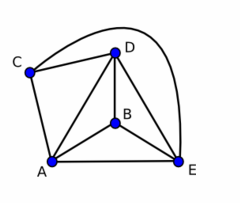
\includegraphics[width=5cm]{K5}
\end{figure}

Similar argument can be said about $K_{3,3}-e$, all of them are isomorphic to each other. Any one of the crossing over edges can be deleted.
\begin{figure}[H]
\centering
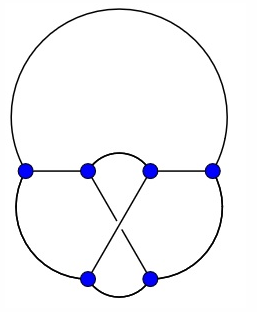
\includegraphics[width=4cm]{K33}
\end{figure}


\item Let $G$ be a bipartite graph and $H$ be a subgraph of $G$. Since $G$ is bipartite there exists a bipartition $V_1, V_2$ of $V(G)$, that is, $V_1, V_2$ is a partition of $G$ such that if $v, w \in V_i,$ where $i = 1, 2$, then $(v,w) \notin E(G)$. In particular, since $V(H) \subseteq V(G)$ we define $V_1' = V_1 \cap V(H)$ and $V_2' = V_2 \cup V(H)$. Note that $V_1', V_2'$ is a partition of $V(H)$, and furthermore it is a bipartition since if $v, w \in V_i'$ , where $i = 1, 2$, then $v, w \in V_i$ as well (since $Vi \subset V_i$), and so $v, w \notin E(H)$ since $v, w \notin E(G)$ and $E(H) \subseteq E(G)$.



\item The graph on 4 vertices with maximum edges is $K_4$. Given that we can provide a planar embedding of $K_4$, every graph on 4 vertices is a subgraph of $K_4$. So, 4 vertices should always be planar as a sub-graph of a planar graph is always planar.




\item The edge set of any subgraph will be a subset of the set of edges in the original planar graph. This means that since edges in the original graphs do not cross, edges in a subset of the original set of edges also do not cross.
 

\item  Given that the graph is 4-regular, degree of each node is 4. $|E|=16$ is given, therefore, we can conclude sum of the degree of all nodes is twice the number of edges, i.e
\begin{align*}
4|V| = 2|E|\\
|V| = 8
\end{align*}
Now using Euler's Formula $|V|-|E|+ r = 2$, we get the number of regions $r=10$.



\item  If $G$ has only one vertex, then this vertex has degree zero. If $G$ has only two vertices, then both vertices have degree at most one. Let $n \geq 3$, where $n$ is the number of vertices. Assume degree of every vertex in $G$ is at least six. Then, $\sum_{v\in V}deg(v) \geq 6n$. We know $\sum_{v\in V}deg (v)=2m$, where $m$ denotes the number of edges. Thus, $2m\geq 6n$ so that $m\geq 3n$. This is not possible because, we know that  $m \leq 3n - 6$. Thus we get a contradiction. Hence G has at least one vertex of degree less than 6. 



\item  If dual of a planar graph is isomorphic to the given graph, we can conclude that number of vertices is the same as the number of regions. Therefore, using Euler's formula for planar graphs, we can conclude that $m=2(n-1)$, where $|E|=m$.


\item 
\begin{enumerate}
\item When $G_1, G_2$ are homeomorphic graphs, then they may be regarded isomorphic except, possibly, for vertices of degree 2. Consequently, two such graphs will have the same number of vertices of odd degree. 

\item If $G_1$ has an Euler trail (and is connected), then $G_1$ has all vertices of even degree, except the end vertices of the trail. From (a) we can conclude that $G_2$ is also connected and has an Euler trail with all vertices having even degree except the end vertices.\\
The converse follows in a similar way.

\item If $G_1$ has an Euler circuit, the $G_1$ ( is connected and) has all vertices of even degree. From (a) we can conclude that $G_2$ is also connected and  has all vertices of even degree. Hence $G_2$ has an Euler circuit as well. \\
The converse follows in a similar way.
\end{enumerate}


\item  Since $C_9$ represents a cycle graph on 9 vertices, we have a unique Hamiltonian path starting from each vertex and moving clockwise (or anti-clockwise). Thus, total number of Hamiltonian graphs are 9.   



\item Every permutation of the vertices given result to a Hamiltonian path when the underlying graph is complete. Therefore, total number of possible permutations are 9!. However, we can observe that there are a pair of permutations that given rise to the same path (i.e start vertex becomes the end vertex and vice versa). Counting each such path only once, we have Total possible Hamiltonian paths to be $\frac{9!}{2}$. 


\item In a complete graph $K_n$, where $n$ is odd, we see that the degree of each node is $n-1$ (even). We also can observe that one Hamiltonian cycle consumes precisely two edges of every vertex. Hence the total number of Hamiltonian cycles are $\frac{n-1}{2}$.




\item Let us prove this by inducting on $n$.\\ 
In the base case $n = 2$, the 2-dimensional hypercube is a square. The length four cycle starts from 00, goes through 01, 11, and 10, and returns to 00.\\
Suppose now that every $(n-1)$-dimensional hypercube has an Hamiltonian cycle. \\ 
Let $v \in \{0,1\}^{n-1}$ be a vertex adjacent to $0^{n-1}$ (the notation $0^{n-1}$ means a sequence of n-1 zeros) in the Hamiltonian cycle in a $(n-1)$-dimensional hypercube. The following is a Hamiltonian cycle in an $n$-dimensional hypercube: have a path that goes from $0^n$
to $0v$ by passing through all vertices of the form $0x$ (this is simply a copy of the
Hamiltonian path in dimension $(n-1)$, minus the edge from $v$ to $0^{n-1}$
), then an edge from $0v$ to $1v$, then a path from $1v$ to $10^{n-1}$ that passes through all vertices of the form $1x$, and finally an edge from $10^{n-1}$ to $0^n$.\\
This completes the proof.

\item Let $x,y \in V$ with $(x,y) \in E$. Therefore $x,y$ are non-adjacent in $\overline{G}$. We also know that the $deg_{\overline{G}}(x)\ =\ deg_{\overline{G}}(y)\ \geq 2n+2-n\ =\ n+2$. \\
Therefore, we see that $deg_{\overline{G}}(x) +  deg_{\overline{G}}(y) = 2n + 4 > 2n + 2 = |V|$.\\ 
By virtue of Theorem 11.9 in the text, we can conclude that there must exist a Hamiltonian cycle.

\end{enumerate}



\end{document}
